\testfile{pgfplotstest.ticks.tex}

\testsection{Scaled ticks}
\testsubsection{false}
\begin{tikzpicture}
	\begin{axis}[scaled ticks=false]
	\addplot coordinates {(-0.00001,2e12) (-0.00005,4e12) };
	\end{axis}
\end{tikzpicture}

\testsubsection{true}
\begin{tikzpicture}
	\begin{axis}[scaled ticks=true]
	\addplot coordinates {(-0.00001,2e12) (-0.00005,4e12) };
	\end{axis}
\end{tikzpicture}

\testsubsection{base 10:3}
\begin{tikzpicture}
	\begin{axis}[scaled ticks={base 10:3}]
	\addplot coordinates {(-0.00001,2e12) (-0.00005,4e12) };
	\end{axis}
\end{tikzpicture}

\testsubsection{real:3.1415}
\begin{tikzpicture}
	\begin{axis}[xtick={0,0.78539,...,10},domain=0:2*pi,enlarge x limits=0,scaled x ticks={real:3.1415}]
	\addplot (\x,{sin(\x r)});
	\end{axis}
\end{tikzpicture}

\testsubsection{real:3.1415 und y = base 10:-2}
\begin{tikzpicture}
	\begin{axis}[xtick={0,0.78539,...,10},domain=0:2*pi,enlarge x limits=0,scaled x ticks={real:3.1415},xtick scale label code/.code={$\cdot \pi$},
		scaled y ticks={base 10:-2},
	]
	\addplot (\x,{sin(\x r)});
	\end{axis}
\end{tikzpicture}

\testsubsection{real:3.1415 und y = real:2}
\begin{tikzpicture}
	\begin{axis}[xtick={0,0.78539,...,10},domain=0:2*pi,enlarge x limits=0,scaled x ticks={real:3.1415},xtick scale label code/.code={$\cdot \pi$},
		scaled y ticks={real:2},
	]
	\addplot (\x,{sin(\x r)});
	\end{axis}
\end{tikzpicture}

\testsection{Minor ticks}

\begin{tikzpicture}
%\tracingmacros=2\tracingcommands=2
\begin{axis}[minor tick num=3]
\smallplotstest
\end{axis}
\end{tikzpicture}

\begin{tikzpicture}
\begin{axis}[minor tick num=1]
\smallplotstest
\end{axis}
\end{tikzpicture}

\begin{tikzpicture}
\begin{axis}[minor tick num=5]
\smallplotstest
\end{axis}
\end{tikzpicture}

\testsubsection{+ Explicit tick marks (non-uniform)}
\begin{tikzpicture}
%\tracingmacros=2\tracingcommands=2
\begin{axis}[minor tick num=5,xtick={0.5,1,2,2.5,3}]
\smallplotstest
\end{axis}
%\tracingmacros=0\tracingcommands=0
\end{tikzpicture}

\testsubsection{+ Explicit tick marks (uniform)}
\begin{tikzpicture}
%\tracingmacros=2\tracingcommands=2
\begin{axis}[minor tick num=5,xtick={-1,...,5}]
\smallplotstest
\end{axis}
%\tracingmacros=0\tracingcommands=0
\end{tikzpicture}

\testsection{Tick placement}
\begin{tikzpicture}
\begin{axis}[
	xtick={-1.5,-1,...,1.5},
	ytick={-0.5,0,...,1.5},
	]
\smallplotstest
\end{axis}
\end{tikzpicture}

\begin{tikzpicture}
\begin{axis}[
	xmin=0,xmax=1,
	xtick={-1.5,-1.25,...,1.5}]
\smallplotstest
\end{axis}
\end{tikzpicture}

\testsubsection{xtick=data}
\begin{tikzpicture}
\begin{axis}[xtick=data,xmajorgrids]
\addplot coordinates {(0,0) (0.4,1) (1,2) (1.2,3) (4,5)};
\end{axis}
\end{tikzpicture}

\begin{tikzpicture}
\begin{axis}[xtick=data,xmajorgrids]
\addplot coordinates {(0,0) (0.4,1) (1,2) (1.2,3) (4,5)};
\addplot coordinates {(0.1,1) (0.5,2) (1.2,3)};
\end{axis}
\end{tikzpicture}

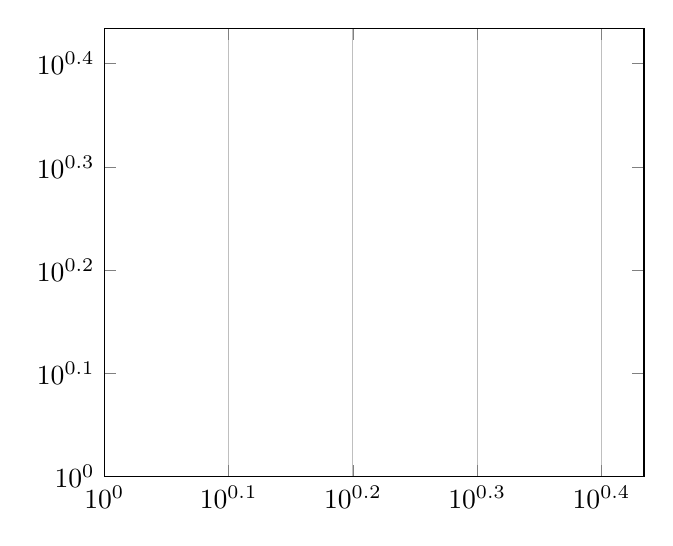
\begin{tikzpicture}
\begin{loglogaxis}[xtick=data,xmajorgrids]
\loglogtestplot
\end{loglogaxis}
\end{tikzpicture}

\testsubsubsection{ytick=data}
\begin{tikzpicture}
\begin{axis}[ytick=data,ymajorgrids]
\addplot coordinates {(0,0) (0.4,1) (1,2) (1.2,3) (4,5)};
\addplot coordinates {(0.1,1) (0.5,2) (1.2,3)};
\end{axis}
\end{tikzpicture}

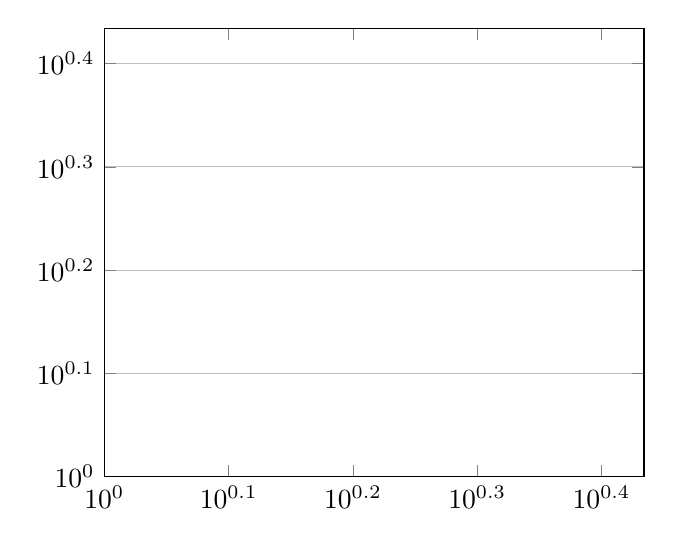
\begin{tikzpicture}
\begin{loglogaxis}[ytick=data,ymajorgrids]
\loglogtestplot
\end{loglogaxis}
\end{tikzpicture}

\testsubsection{ticks on axis rectangle}
First plot: default tick style; second plot: red, third: 'help lines'

{\pgfplotsset{every axis/.append style={
	enlargelimits=false,
	xmin=-40,xmax=40,ymin=-40,ymax=40,
	xtick={-40,0,40},
	ytick={-40,0,40}
}}%
\begin{tikzpicture}
\begin{axis}[
]
\addplot coordinates {(-40,-40) (40,40)};
\end{axis}
\end{tikzpicture}
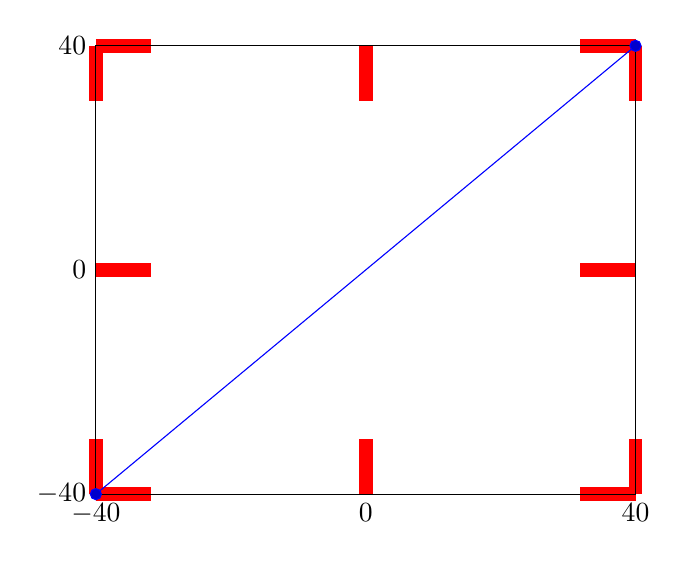
\begin{tikzpicture}
\begin{axis}[
	tick style={red,line width=5pt,major tick length=20pt},
]
\addplot coordinates {(-40,-40) (40,40)};
\end{axis}
\end{tikzpicture}
\begin{tikzpicture}
\begin{axis}[
	tick style={help lines},
]
\addplot coordinates {(-40,-40) (40,40)};
\end{axis}
\end{tikzpicture}
}

\testsubsection{modified labels}

{
\pgfplotsset{every axis label/.style={}}
\pgfplotsset{every axis x label/.style={
    at={(0.5,1)},
    above,
    yshift=+15pt}}
\pgfplotsset{every axis y label/.style={
    at={(1,0.5)},
    xshift=+35pt,
    rotate=90}}

\begin{tikzpicture}
\begin{axis}[
	xlabel=$x$ axis,
	ylabel=$y$ axis,
	xmin=0,xmax=1,
	tickpos=right,
	xtick={-1.5,-1.25,...,1.5}]
\smallplotstest
\end{axis}
\end{tikzpicture}
}

\begin{tikzpicture}
\begin{axis}[
	xlabel=$x$ axis,
	ylabel=$y$ axis,
	xmin=0,xmax=1,
	tickpos=both,
	xtick={-1.5,-1.25,...,1.5}]
\smallplotstest
\end{axis}
\end{tikzpicture}

\testsection{Tick label assigment tests}
\testsubsection{Using xticklabel and xtick}
\begin{tikzpicture}
\begin{axis}[
	xtick={-1.5,-1,...,1.5},
	xticklabel={%
		\ifcase\ticknum	$-1\frac12$%
		\or				$-1$%
		\or				$-\frac12$%
		\or				$0$%
		\or				$\frac12$%
		\or				$1$%
		\or				$1\frac12$%
		\else			$\tick$%
		\fi
	}
]
\smallplotstest
\end{axis}
\end{tikzpicture}

\testsubsection{Showing ticknum verbatim}
\begin{tikzpicture}
\begin{axis}[
	every tick label/.append style={font=\footnotesize},
	xticklabel={\#\ticknum = \tick},
	yticklabel={\#\ticknum = \tick},
]
\smallplotstest
\end{axis}
\end{tikzpicture}

\testsubsection{Using xticklabels}%
\begin{tikzpicture}
\begin{axis}[
	xtick={-1.5,-1,...,1.5},
	xticklabels={%
		$-1\frac 12$,
		$-1$,
		$-\frac 12$,
		$0$,
		$\frac 12$,
		$1$}
]
\smallplotstest
\end{axis}
\end{tikzpicture}

\testsubsection{With xtick labels and commas by hand}
\begin{tikzpicture}
\begin{axis}[
	xtick={-1.5,-1,...,1.5},
	xticklabels={%
		{-1,5},
		-1,
		{-0,5},
		0,
		{0,5},
		1,
		{1,5}}
]
\smallplotstest
\end{axis}
\end{tikzpicture}

{
\testsubsection{Only with auto number formatting options; different for x and y}
%\tracingmacros=2\tracingcommands=2
\begin{tikzpicture}
\begin{axis}[
	xtick={-1.5,-1,...,1.5},
	x tick label style={/pgf/number format/use comma},
	y tick label style={/pgf/number format/.cd,use comma,fixed zerofill,precision=3},
]
\smallplotstest
\end{axis}
\end{tikzpicture}
}

\testsubsection{Using yticklabels in logplot}%
{
\def\tickformat#1{1e#1}%
\begin{tikzpicture}
\begin{loglogaxis}[
	ytick={1e-8,1e-7,1e-6,1e-5,1e-4,1e-3,1e-2,1e-1,1e0,1e1},
	yticklabels={%
		\tickformat{-8},
		\tickformat{-7},
		\tickformat{-6},
		\tickformat{-5},
		\tickformat{-4},
		\tickformat{-3},
		\tickformat{-2},
		\tickformat{-1},
		\tickformat{-0}}
]
\loglogtestplot
\end{loglogaxis}
\end{tikzpicture}
}

\testsection{Tick/Tick-Label placement log plots}
\testsubsection{ytickten}
\begin{tikzpicture}
\begin{loglogaxis}[
	%xmin=0.99e2,xmax=1e4,
	ytickten={-5,-4,-3.6,-3,-2,-1,0},
	yticklabel={
		\ifnum\ticknum=2	
			$\rightarrow$
		\else
			\axisdefaultticklabellog
		\fi
	}
]
\loglogtestplot
\end{loglogaxis}
\end{tikzpicture}

\testsubsection{ytick}
\begin{tikzpicture}
\begin{loglogaxis}[
	ytick={1e-5,1e-4,0.000251188643,1e-3,1e-2,1e-1,1e0},
]
\loglogtestplot
\end{loglogaxis}
\end{tikzpicture}

\testsubsection{extra y ticks}
\begin{tikzpicture}
\begin{loglogaxis}[
	extra y ticks={0.000251188643,5e-2},
]
\loglogtestplot
\end{loglogaxis}
\end{tikzpicture}

\testsubsection{extra x and y ticks, linear plot}
\begin{tikzpicture}
\begin{axis}[
	xmin=0,xmax=3,ymin=0,ymax=15,
	extra y ticks={2.71828},
	extra y tick labels={$e$},
	extra x ticks={2.2},
	extra x tick style={grid=major,/pgfplots/tick label style={rotate=90,anchor=east}},
	extra x tick labels={Cut}
]
	\addplot (\x,{exp(\x)});
	\addlegendentry{$e^x$}
\end{axis}
\end{tikzpicture}
